
\chapter{Individual refactored views}

In a project with multiple developers situations may arise where you need to make a change to the structure of the source code. This becomes a problem if you also want to limit the impact other developers.  Maintaining your own independently refactored view of the source code could be valuable in these circumstances. 

\section{The problem}
\begin{description}
  \item [Repeated structure changes for other software developers.]   
    Imagine a situation where you are working jointly on a project with other people. Since you want to collaborate on different aspects of the same source code you have set up the project in a merge based version control system.  You have checked out your own copy of the code so that you can work on the source code without interfering with any of the changes others are making. You notice that you they are going to have to refactor the code before you add any of your changes.  This would be a fair judgement call as Fowler claims that the main time to do refactoring is before making any changes \cite{Fowler1999}. You complete your changes and check in your code back into the version control system.  While you are doing this other people have been working on the code.  If you manage to check in your code before anyone else you will not need to merge any of your changes.  Anybody who checks in after you however, could have a merge conflict.  Some conflicts that they experience could be because the changes you made directly compete with the changes you have made. Potentially more conflicts would occur between the changes they have made and the refactoring that you have completed. This is because a refactoring often makes a large amount of global changes to the source code.

    \begin{figure}
    \begin{center}
    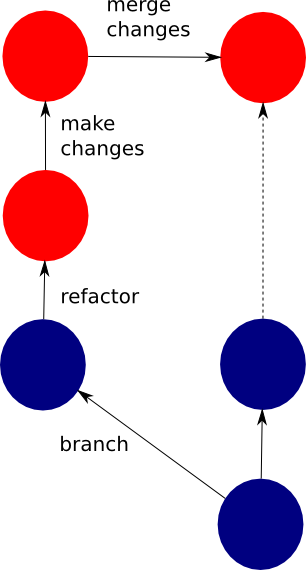
\includegraphics[scale=0.5]{refactorCheckIn}
    \end{center}
    \caption{Merging changes with refactored code also merges any refactoring}
    \end{figure}

    As shown in figure the difficulty lies in the fact that not only the functionality that you have added is checked in but also the changes brought about by refactoring.  These refactored changes have not changed how the program functions but have simplified and tidied the code to make the addition of your changes easier. There are some occasions where you may want to avoid changing other peoples code in such a dramatic fashion.  

    In some conditions refactoring is only required to simplify the code to implement a small change as opposed to cleaning up the entire code base.  This partial refactoring is likely if the code base is large. According to Melina et. al. \cite{Milea2014} refactoring is a challenge when the code base is large. By definition refactoring does not any functionality but changes the source code. This means that the code previous to being partially refactored has the equivalent functionality to the code after the partial refactoring.

    By checking in your refactoring code you are forcing others to comply with your vision about how the code should be structured.  This occurs even though you could have no awareness about what changes to the code others have made or intend to make.  Everyone who attempts to check in their code after you will need to merge into a restructured code source that they are unfamiliar with.  The potential for merge based bugs and time wasted doing unnecessary merging increases.

    % then created a branch
    % If they attempt to check-in their changes there is the possibility a
    % conflict with any of your changes.
    % 
    % You also need to refactor the code to do your work but both of the
    % refactorings are different because they clarify or highlight different
    % aspects of the source code.
    % 
    % If there is some refactoring before any changes are made when the code 
    % is
    % merged with the original project (often called the trunk project) both
    % the changes and the refactored code are checked in.
  \item [Difficulty if there are multiple check-ins.] 
    When there is a large change on a separate branch with many development milestones it is desirable to have the ability to submit your code periodically.  This could be done to ensure that there is not too much divergence between the separate branch and other development projects. The desire to regularly merge the code makes the issue we have discussed even worse. Currently if you have a project where there are periodic check-ins for each development milestone there will be a large impact each time there is a commit. This is because the refactoring for the large refactored project is imposed upon others each time it is merged.

    One of the ways this can be dealt with is by creating separate branches for different projects however this has some issues with merging when working on two or more projects simultaneously.  In order to minimise the amount of divergence it is advisable to merge each of the branches with the trunk often.  If there has been global refactoring changes introduced by one project being merged the merge will be worse for any of the remaining branches when they are checked in.  Instead of having an issue merging at the check-in level we now have an issue at the merging of branches.  As these changes will occur less often than checking in the code, the code will possibly have more divergence.  This divergence is likely to cause more rather than less merge issues at the expense of having to merge less often.
  \item [Differences in how code is understood.]    
    According to  Kerievsky a reason for refactoring code is to better understand it \cite{Kerievsky2004}. The very act of going through the source code and reprocessing it in a clearer form can help with the understanding of it. This would suggest that developers tend to leave the code in a difficult to understand state or that different developers understand things differently.
    Kerievsky also relates a tale about how the lack of knowledge of patterns making a particular refactoring look a lot more complex \cite{Kerievsky2004}. The different perspectives meant that the programmer he refers to as John has a differing opinion that the refactored code was not an improvement. This shows that it is not just different functionality that influences the need to refactor but sometime the knowledge and experience of the developers themselves. It is often the case that two developers could have different views about what is an appropriate refactoring. This could be because each person brings different skills, notices different issues and has a preferred way of visualizing a problem and solution.
  \item [Version control systems not being aware of changes in the order.]
    One of these changes which is not catered for by current version control systems is the changes of order.  The first person to check-in their code will have no issue as the version control system assumes that all the changes are simply a new revision.  When the second person attempts to reconcile their view there is the possibility of having unnecessary conflicts.  A lot of these conflicts will be with refactored code which although works the same has a different structure.
\end{description}







\section{Benefits of individual refactored views}
We want to be able to maintain private views or separate branches that can have different but equivalent refactoring. Different structures of code that function the same way a number of features that could be of interest.

\begin{description}

  \item [Reduced interference with other software developers.]   
  One benefit is that it is possible to keep the structure of code that each software developer works on consistent.  The location of methods and variables are more likely to remain in the place the software developer left them even if a merge occurs.
  By maintaining two differently refactored view it allows software developers to work on the same programming project to freely refactor with minimal interference to others.
  If two software developers refactor the code that they are able to hold their own individual refactoring with reduced changes when they are merged.
  The reduced changes would also mean that there will be less unnecessary merge conflicts when merging code.
  
  \item [The number of changes is reduced when merging] 
  The number of changes when merging is reduced if you omit any changes that don't also have any change in behaviour.  This in turn means that there is less chance for there to be a merge conflict.
  
  \item [The ability to have comment tied to a specific view.] 
  It would be possible to have comments that are not considered when doing a merge. This would be a benefit if there are comment that are specific to a branch and that are not necessary to share.  This would allow a programmer to keep a lot more personal notes.  The risk of having so many comments from others that it is hard to see the code is reduced. By being able to identify that a block of text comment is a new addition

\end{description}

% Can it help with throwaway code or code uede for debugging
% 
% 
% When these branches are merged we want to make sure that any source code 
% that is equivalent but refactored is not merged to the view we are merging 
% into. Any source code that changes the behaviour however is considered in 
% the merge.
% 
% We also want to be able to further classify more complex operations in a 
% change set than insert, delete and modify.  When JGit compares files with 
% each other because they are structured it can determine if the file has been 
% moved to a different location in the tree.  At this level JGit can also 
% detect copies and renames.  However once JGit starts comparing source code 
% it loses this structural information.  By giving JGit some idea about the 
% structure in the file it can determine these item at the finer granularity 
% of sections of code rather than at a file basis.


\section{Ways individual refactored views could be achieved}
There are a number of ways we have considered about how to provide differently reafactored views that have the same functionality.

\begin{description}
  \item [Comparing differences using a non-ordered comparison algorithm.]   
    Instead of using the Longest Common Subsequece based approach we could instead use a non-ordered comparison.  The easist way to consider this concept is that the LCS algorithm compares two lists whereas a non-ordered algorithm is a bit more like comparing sets of items. The items within the set will still be ordered.

    \begin{algorithm}[H]
    \SetAlgoLined
    \While{There are elements on both sides that match}{
    Create a histogram of remaining elements\;
    Select one of the elements that occurs in both sides the least but not zero times\;
    \While{There is an element below the selected one that matches on both sides}{
    Remove element from list of elements to compare, as it matches\;
    }
    \While{There is an element above the selected one that matches on both sides}{
    Remove element from list of elements to compare, as it matches\;
    }
    Remove selected element from list of elements to compare, as it matches\;
    }
    \caption{A non-ordered comparison algorithm}
    \end{algorithm}


    The problems with using this approach to reconcile to different ordered sets is that comparison whould not know the difference between what needs to strictly remain in order and what is allowed to be in a different order. If the version control system has an understanding of a particular computer language it is much easier to determine what items can be moved without changing functionality and which ones need to stay in the same order. 
  \item [Normalising the source code before placing it in the version control system.]
    Before placing the item into source control it could be transformed into an agree upon format. Before allowing a merge on a block of code each the views could transform the block of code using the same method and compare it with the equivelent block of code that in the version control system. If the transformed code is the same then there is no need to merge.
  \item [Storing additional infomation in the version control system.]
    By storing additional information within the version control system different views could be managed and recreated.
    This concept is very similar to Ekmans plugin for eclipse that maintains a record different refactorings in addition to the source code \cite{Ekman2004}.

    The problem with this is that it would have to store information about every view that was differently refactored.  In a distributed version control system especally an online one the number of distinct views could be large and change often.   
  \item [Using a tool like JDime solely as a method of comparision.]
    As mentioned earlier there are a number of reasons why JDime cannot currently be used as a method of keeping two different refactored views. If changed however it could still be useful.  One idea we had was to attach it to Git and solely use it to detect equivalent pieces of java source code.
\end{description}


